\section{Schildererkennung}
\label{sec:schildererkennung}

F\"ur unsere selbst gew\"ahlte Zusatzaufgabe sollte das Fahrzeug, "ahnlich wie ein Mensch, die Verkehrsschilder auf dem Rundkurs wahrnehmen k"onnen und diese visuell erkenntlich machen.

\begin{figure}[h]
	\centering
	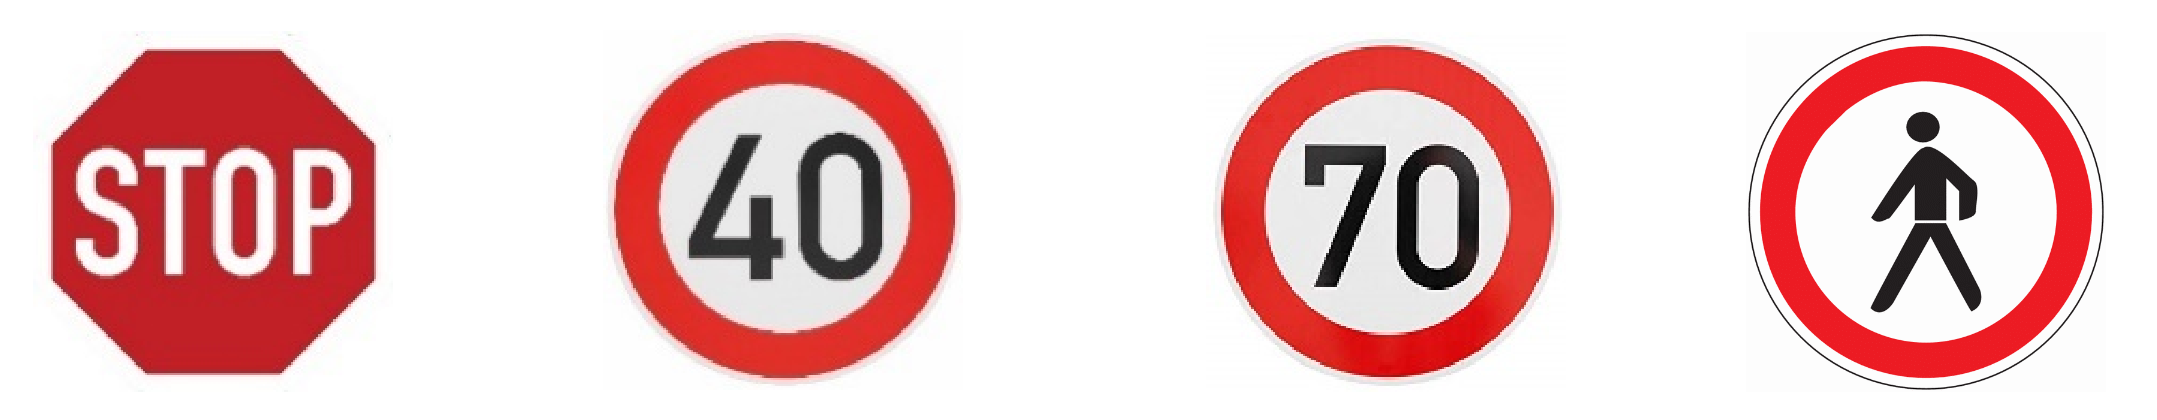
\includegraphics[width=0.9\textwidth]{images/Verkehrszeichen}
	\caption{Verkehrszeichen}
	\label{fig:verkehrszeichen}
\end{figure}

\subsection{Implementierung}
Um diese Motivation umsetzen zu k"onnen, haben wir ein k"unstliches neuronales Netz gew"ahlt. Dieses ist biologischen Prozessen nachempfunden und wird vermehrt im Bereich des maschinellen Lernen von Bildern verwendet. Das neuronale Netzwerk YOLO (You Only Look Once \cite{darknet13}) ist ein State-of-the-art real-time Objektdetektor
%TODO: dieses "state-of-the-art" ist eigentlich nur ein Kampfbegriff für "neuster Stand" und sagt m.Mn. nach nichts über die Technologie aus (Frederic)
basierend auf dem \textbf{Darknet}, einem Machine Learning Framework basierend auf C und CUDA.
Die allgemeine Herausforderung eines Objektdetektors besteht darin, das Objekt im Bild zu detektieren und anschliessend zu klassifizieren. Der Vorteil des YOLO Netzes besteht neben der gleichzeitigen Lokalisierung \& Klassifizierung mehrerer Objekte in einem Bild, dass es auf unerwartete Eingaben sehr adaptiv reagiert und somit f"ur weniger Ausf"alle des Erkennungssystems sorgt. Dies erm"oglicht uns auch mehrere Verkehrsschilder auf einmal in einem Bild zu erkennen, wobei das aktuell n"achstgelegene Schild selektiert wird.

Der erste von uns verwendete Ansatz war die Benutzung der aktuellen Version YOLOv3. Es stellte sich jedoch heraus, dass die eingeschr"ankte Hardware auf dem Fahrzeug der limitierende Faktor ist und der ROS Wrapper nicht das aktuelle YOLOv3 verwenden kann. Daher wurde aus Gr"unden der Performance die YOLOv2 Tiny Version verwendet, welche eine reduzierte Variante des YOLOv2 darstellt und eine geringere Pr"azision in der Erkennung hat.

\subsection{Aufbau des neuronalen Netzes}
\label{sec:cnn_aufbau}
Ein k"unstliches neuronales Netz besteht aus mehreren Neuronen, die "uber mehrere Schichten (Layer) mit einander verbunden sind (siehe Abb \ref{fig:neunet}). YOLO ist ein Single CNN (Convolution Neuronal Network, ein faltendes neurales Netz, das einen Input in Form einer Matrix verarbeitet),
welches aufgrund seines schlanken Aufbaus eine enorme Schnelligkeit erm"oglicht. Es verarbeitet ein Bild und detektiert dabei mehrere Objekte (Single Shot Detector). Andere Netze ben"otigen f"ur diese vergleichbare Detektion mehrere Durchl"aufe - jeweils einen Durchlauf f"ur das Detektieren der Objekte und jeweils eine Iteration pro gefundenem Objekt zur Klassifikation (z.B. R-CNN, R-FCN).
%TODO: Referenzen (Frederic)

\begin{figure}[h]
	\centering
	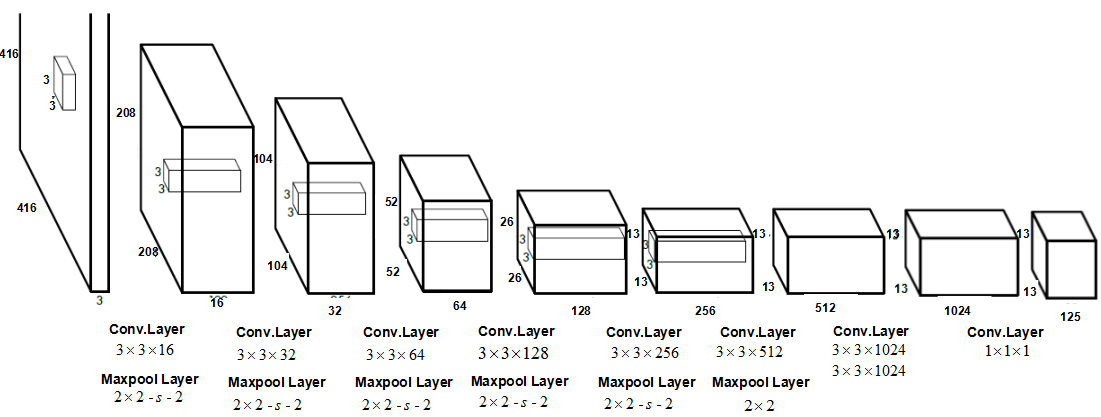
\includegraphics[width=0.90\textwidth]{images/aufbauskizze}
	\caption{Aufbauskizze}
	\label{fig:neunet}
\end{figure}

Das YOLO CNN besteht aus mehreren Convolutions (Faltungsschichten) und Maxpool Layers (Aufteilung des Input in Rechtecke mit Maximumsbestimmung) zum Subsampling.
%TODO: "Convolution", "Maxpool Layers", "subsampling" -> alles Begriffe, mit denen der Leser in aller Regel nichts direkt anfangen kann (Frederic) @ edit DP Subsampling zum herunterskalieren, 
Diese reduzieren die Dimension der Eingabedarstellung Schritt f\"ur Schritt so,
%TODO: was für "Annahmen"? -> das muss erklärt werden! (Frederic)
dass der Rechenaufwand erheblich reduziert wird. Am Ende befindet sich ein $13*13*45$ Quader, der die Klassifikation und Detektion des verarbeiteten Inputs "ubernimmt. Die Bedeutung der Dimensionen wird nachfolgend erkl\"art:
%TODO: "Wofür stehen diese Dimensionen" -> ist eine Frage, kann hier nicht so mit Doppelpunkt verwendet werden (Frederic) @edit DP

Das 13 x 13 Grid beschreibt die Gr"osse eines Rasters, in das das Bild unterteilt wird. Die Tiefe 45 l"asst sich in zwei Werte aufteilen. Zum einen die Startposition der Boundingbox(pc) sowie dessen H"ohe und Breite (bx, by, bh, bw).  Zum anderen die IoU (Intersection over Union). Dieser Wert gibt das Verh"altnis zwischen der "uberlappenden Fl"ache und der vereinigten Fl"ache an. Veranschaulicht ist dies ein Ma\ss \ daf\"ur, wie gut eine Detektion mit der realen Position des Objekts vergleichbar ist (siehe Abb. \ref{fig:stoppschild}). Das neuronale Netz berechnet den IoU-Wert und gibt somit ihre Treffergenauigkeit an. Die Anzahl unserer 4 Objektklassen (STOP, Fussg"anger, 40, 70),  werden der Tiefe des Quaders noch hinzuaddiert,
%TODO: was sind (unsere) "Objektklassen"? Was is die "Tiefe"? (Frederic) @edit DP
sodass der Quader nachfolgende Gr"osse besitzt:

%TODO: ZUM ABSCHNITT: Das klingt gerade alles für mich noch sehr schwammig, es werden haufenweise Begriffe eingeführt, die man als Fachfremder (jemand, der nichts mit neuronalen Netzwerken zu tun hat) nicht versteht... Z.B. die "Tiefe" bzw. der Begriff "Quader" kommen ohne Zusammenhang. (Frederic)
%TODO: Ich würde entweder alles viel detaillierter erklären oder das meiste rausschmeißen und die Beschreibung des neuronalen Netzes stattdessen ganz allgemein und einfach halten. (Frederic)

\begin{equation}
\begin{bmatrix}13 * 13 (Grid)\end{bmatrix} * \begin{bmatrix}5 * [ 5 (Boundingbox) + 4 (Objektklassen)]\end{bmatrix}
\end{equation}

\begin{figure}[h]
	\centering
	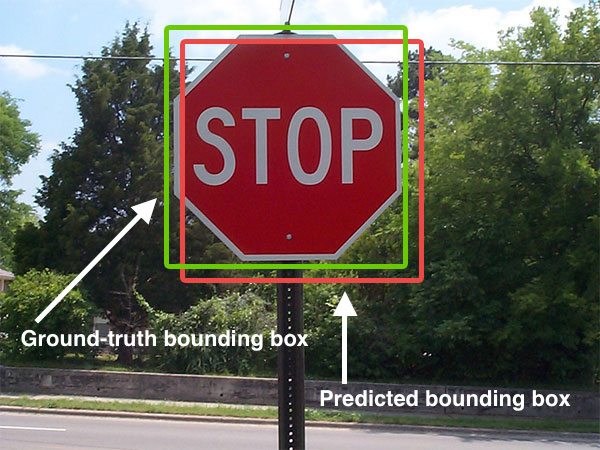
\includegraphics[width=0.65\textwidth]{images/stoppschild}
	\caption{Erkanntes Stoppschild mit Boundingboxes}
	\label{fig:stoppschild}
\end{figure}

\subsection{Ablauf der Detektion}

\begin{figure}[h]
	\centering
	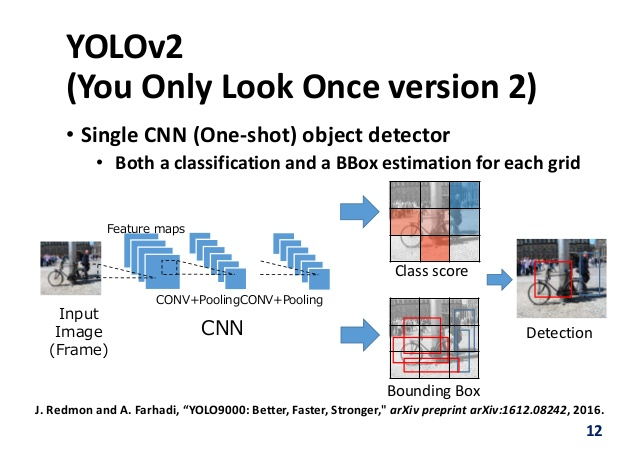
\includegraphics[width=0.9\textwidth,trim={1.2cm 1cm 1cm 6.3cm},clip]{images/yolo_schaubild}
	\caption{Ablaufprozess des neuronalen Netzes YOLO}
	\label{fig:yolo}
\end{figure}

Die einzelnen Frames der Webcam werden dem neuronalen Netz als Input zur Verf"ugung gestellt. Somit verwendet das YOLO Netz ein vollst"andiges Bild zur Erkennung, das es uns erm"oglicht, weniger Hintergrundfehler zu erhalten. Au\ss erdem wird der Kontext der Objekte mitbetrachtet. Das gesamte Bild wird in einzelne Grids aufgeteilt und dem CNN "ubergeben. Pro Grid kann ein Objekt erkannt werden. Damit man auch mehrere Objekte detektieren kann, die eventuell weiter entfernt sind, verwenden wir abweichend vom Standard Grid (32 x 32) eine Gr"osse von 13 x 13 Pixel. Der komplexe Prozess des CNN l"asst sich vereinfacht durch diesen Ablauf beschreiben:

\begin{enumerate}
	\item Bildinput wird auf Eingangsgr"o\ss e des Netzes angepasst (416 x 416 Pixel)
	\item Durchlaufen des Convolutional Network
	\item Non-max Suppression (Pro Objektregion wird das Objekt nur einmal erkannt, reduziert Redundanzen) 
\end{enumerate}

Das detektierte Objekt mit der h"ochsten "Ubereinstimmung (> 60\%) mit unseren Objektklassen wird im Bild durch eine bunte Boundingbox gekennzeichnet und dem entsprechenden Label versehen.

\begin{figure}[h]
	\centering
	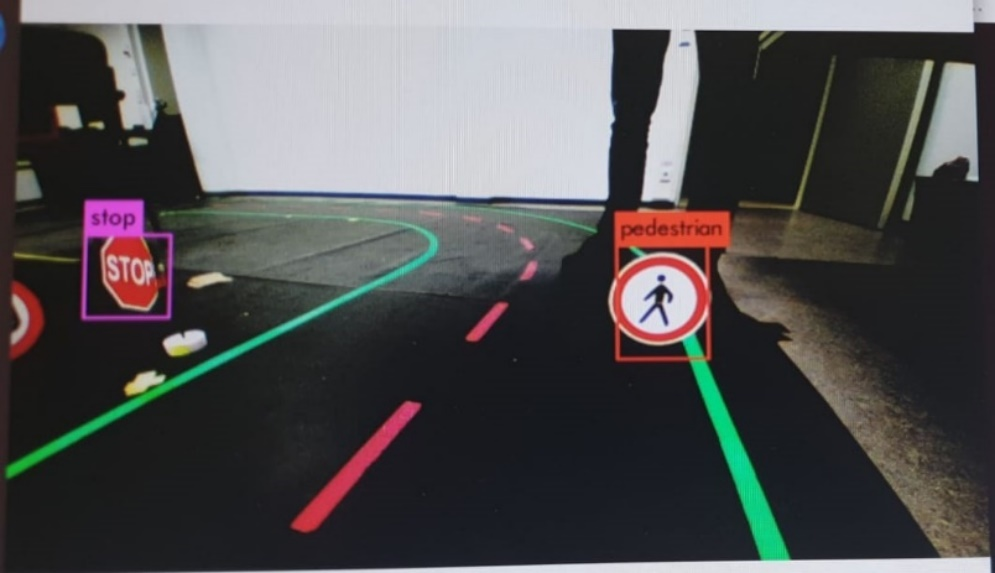
\includegraphics[width=0.9\textwidth,trim={0.5cm 1cm 1cm 1cm},clip]{images/boundingboxes}
	\caption{Erkannte und markierte Schilder auf dem Rundkurs}
	\label{fig:boundingboxes}
\end{figure}

Anschlie\ss end wird das Ergebnis der Verkehrsschildererkennung "uber das ROS-Netzwerk gepublished. Um das YOLO Netz auf dem Fahrzeug auszuf"uhren verwenden wir ein angepasstes Interface von leggedrobotics \cite{leggedrobotics}. Es l"adt die Bilder der ROS-Node \texttt{webcam\_publisher} ein und startet die Verkehrsschildererkennung mit dem selbsttrainierten Netzwerk "uber ROS. "Uber das ROS Netzwerk k"onnen nun die Anzahl der erkannten Objekte (Topic: \texttt{object\_detector}), die Position dieser (Topic: \texttt{bounding\_boxes}, ein Array mit Boundingboxen in Pixelkoordinaten) und das resultierende Bild mit den erkannten Detektionen (Topic: \texttt{detection\_image}) ausgelesen werden.

\subsection{Training}

Das Neuronale Netz wurde bereits mit dem Pascal VOC Datensatz (Visual Object Classes, enth"alt standardisierte Bilder zur Objektdetektion)
%TODO: was ist "VOC"? -> erklären, kennt der Leser nicht (Frederic) @edit DP
per Transfer Learning vorverarbeitet. Die Ergebnisse eines fertig trainierten Netzes werden dabei auf ein neues Netz "ubertragen. Die Layer/Neuronen des Netzes werden danach mit dem neuen Datenset trainiert.
%TODO: schlechter Stil, hier in Klammern ganze Sätze einzuschieben und danach den vorherigen Satz noch zu beenden, verstehe nicht, was gemeint sein soll (Frederic) @edit DP
Dies erm"oglichte es uns, ein vortrainiertes Netz zu verwenden, welches bereits f"ur die Objekterkennung konfiguriert ist und durch unseren Datensatz optimiert wird. Wir haben das Netz mit dem Supervised-Learning-Verfahren trainiert (ein "uberwachtes Lernen, bei dem die Ergebnisse des Lernprozesses mit den Referenzergebnissen verglichen werden).  Zu diesem Zweck wurde der Datensatz in Trainings- und Testdaten aufgeteilt. Unser Datensatz besteht aus 1700 selbstaufgenommenen Verkehrsschildern "uber die Webcam des Autos, ca. 400 Bilder pro Objektklasse (STOP, Fussg"anger, 40, 70), die mit dem Tool Yolo\_mark \cite{Yolo_mark} gelabelt wurden.

Der Trainingsdatensatz wird als Input f"ur das Netz verwendet. Diese passieren das Netz "uber die Neuronen durch die verschiedenen Layer zum Output Quader (Forward Pass). Das Ergebnis der Berechnung wird mit dem bekannten Ergebnis des Testdatensatzes verglichen und der Fehler/Abweichung berechnet. Dieser Fehler wird durch das Netzwerk r"uckw"arts propagiert (Backward Pass) und jedes Neuron entsprechend im Verh"altnis zur Learning Rate (0,001) angepasst. Somit wird das Netz nur minimal ver"andert, um ein Overshooting (zu gro\ss e Ver"anderungen, z.B. bei einer Fehlfunktion) zu verhindern. Dieser Ablauf beschreibt eine Trainings-Epoche des Netzes.  Solch eine Epoche wird zum Trainieren mehrere 1000 Mal ausgef"uhrt um ein zufriedenstellendes Ergebnis des Trainings zu erhalten. (Darauf wird in folgendem Abschnitt noch genauer eingegangen.) Das verwendete Darknet YOLO Datenset besteht aus nachfolgenden Elementen:

\begin{itemize}
	\item \textbf{.cfg} enth"alt die Strukturdefinition des neuronalen Netzes (Layers, Gr"osse des Inputs, Gridgr"osse, Learningrate, ...)
	\item \textbf{.weights} enth"alt die erlernten Gewichte
	\item \textbf{.yaml} Referenzfile zu den Weights und Config, inklusive Erkennungsrate (Threshold)
	\item \textbf{.data} Referenzfile zu Trainingsdaten \& Beschriftung
\end{itemize}

\subsection{Validierung}
Die G"ute/Genauigkeit der richtigen Detektion eines Objektes wird durch folgende Werte bestimmt:

\begin{figure}[h]
	\centering
	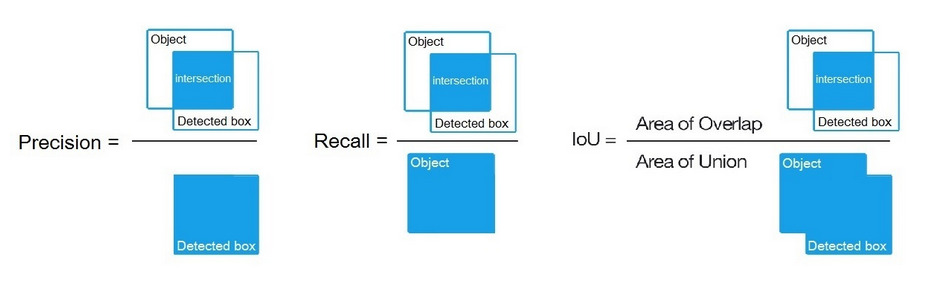
\includegraphics[width=1.0\textwidth]{images/genauigkeit}
	\caption{G"utebestimmung}
	\label{fig:genauigkeit}
\end{figure}

Die Detektionsfl"ache wird mit der tats"achlichen Fl"ache eines Objektes vergleichen und der Grad der "Ubereinstimmung bestimmt. W"ahrend des Trainings kann man in Abb. \ref{fig:training} erkennen, dass neben dem rapide absinkenden Fehler (Loss) in blau, der mAP-Wert (mean average precision) in rot, mit Laufe der Iterationen stetig steigt und sich der 100\% Linie ann"ahert (Convergence). Ab ca. 93\% schwankt der Wert immer mehr und n"ahert sich dem Wert 1 an. Dieser Bereich unterscheidet sich signifikant vom restlichen Graphen und deutet auf Overfitting hin.

Overfitting beschreibt das Problem, dass ein Netz beim Trainieren alle bereits bekannten Bilder sehr oft als Input erhalten hat und diese eher auswendig lernt anstatt des Konzepts des Bildes zu lernen. Um dieses ungewollte Verhalten zu minimieren werden beim Training in jedem Layer des Netzwerks eine gewisse Anzahl an Neuronen ausgelassen (Dropout). Zus"atzlich werden die Bilder zur Validierung in einem Trainingsdatenset und Testdatenset aufgeteilt mit dem Verh"altnis 70 zu 30.
%TODO: was ist das für ein Verhältnis bzw. was gibt das an? (Frederic) @edit DP

\begin{figure}[h]
	\centering
	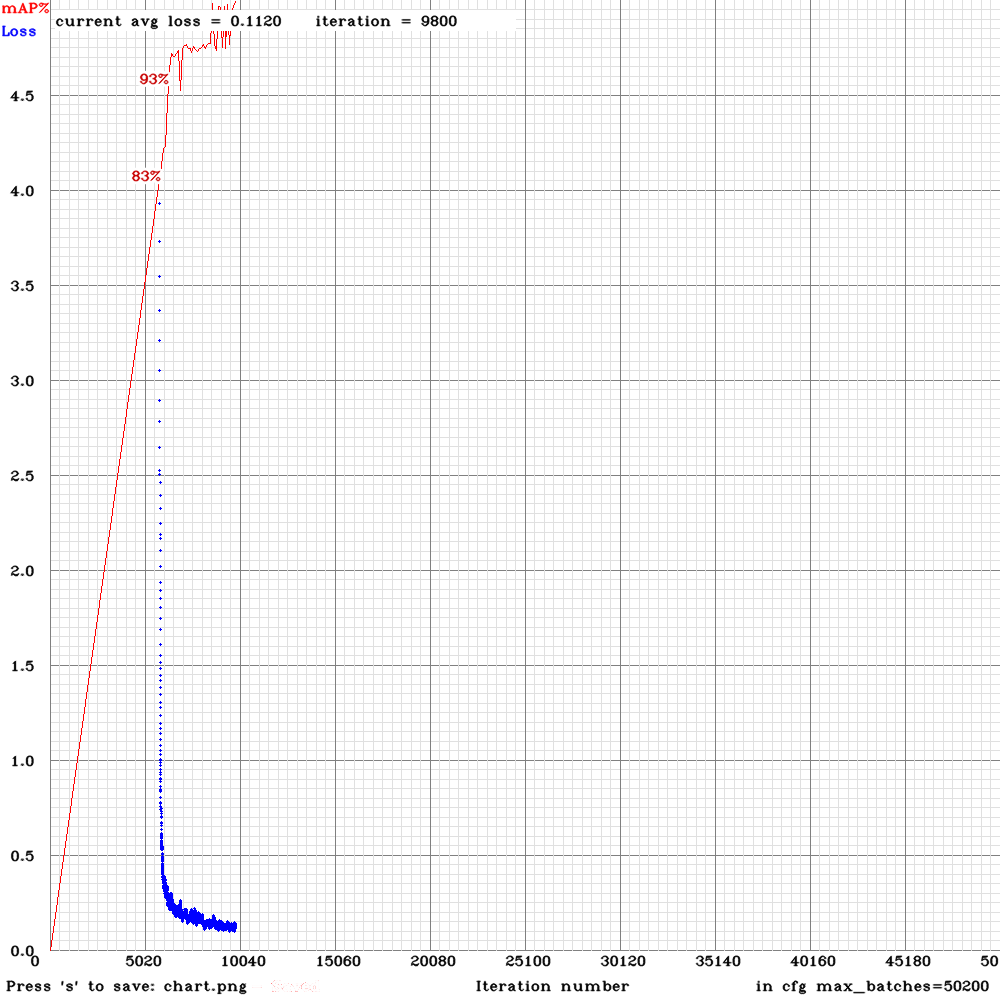
\includegraphics[width=0.85\textwidth]{images/training}
	\caption{Trainingsverlauf}
	\label{fig:training}
\end{figure}

Nach dem Training k"onnen wir die jeweiligen Objektklassen (STOP, Fussg"anger, 40, 70) mit einer Wahrscheinlichkeit von 90\% bzw. bei dem Schild 70 mit 77\% richtig erkennen. Der IoU (siehe Abschnitt \ref{sec:cnn_aufbau}) Wert liegt bei 63\% und der mAP bei 87\%. (Siehe Abb. \ref{fig:ergebnis}).

\begin{figure}[ht]
	\centering
	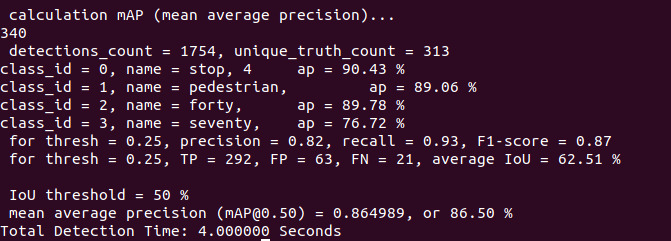
\includegraphics[width=0.9\textwidth]{images/ergebnis}
	\caption{Ergebnisse des Trainings}
	\label{fig:ergebnis}
\end{figure}

\subsection{Optimierungen}
Im zuk\"unftigen Versionen wird der ROS-Wrapper in der Lage sein mit der aktuellen Yolov3 Version interagieren zu k"onnen, sodass wir eine noch schnellere, pr"azisere und ressourcenschonendere Verkehrsschilderkennung verwenden k"onnen.

Die Genauigkeit der Schildererkennung kann durch den Datensatz von 1000 gelabelten Bildern pro Klasse verbessert werden.

Die allgemeine Leistungssteigerung der Fahrzeughardware w"urde die Erkennung von vielen weiteren digitalen bzw. dynamischen Wechselverkehrszeichen erm"oglichen, sodass das Fahrzeug auch in besonderen Situationen, zum Beispiel bei Sperrung einer Fahrbahn in einer Baustelle, entsprechend reagieren kann.
%TODO: was für "digitale" bzw. "dynamische" Schilder? (Frederic) @edit Wechselverkehrszeichen ist der Fachbegriff für digitale Schilder die zum Beispiel auf der Autobahn ueber der Fahrbahn haengen und per LED Matrix mit beliebiegen Tect bzw. Schildern beschriftet werden koennen
%TODO: warum gerade "Baustellsituationen"? würde ich eher weglassen (Frederic)

\begin{figure}[ht]
	\centering
	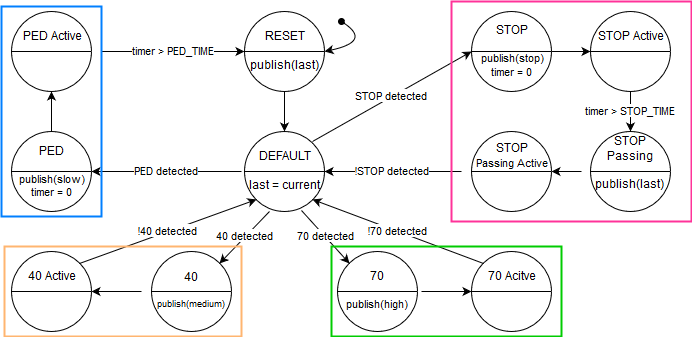
\includegraphics[width = 1\textwidth]{images/StateMachine.png}
	\caption{Zustandsautomat f\"ur die Schildererkennung}
	\label{fig:zustandsautomat}
\end{figure}

\subsection{Reaktion auf erkannte Schilder}
Momentan erkennt das neuronale Netz vier Schilder, doch das Roboterauto reagiert noch nicht auf diese und erkennt sie nur. Das Team hat bereits einen Zustandsautomaten f\"ur die Weiterverarbeitung der Schildererkennung entwickelt (siehe Abbildung \ref{fig:zustandsautomat}) und in C++ realisiert.

Wenn das neuronale Netz ein Schild oder mehrere Schilder erkennt, dann werden diese \"uber ein ROS-Topic ver\"offentlicht. Diese erkannten Schilder werden zun\"achst darauf \"uberpr\"uft, welches das n\"achste Schild im Abstand zum Roboterauto ist und ob der Abstand zu dem Schild klein genug ist, um darauf reagieren zu m\"ussen. Falls dies der Fall ist, so wird das entsprechend n\"achste Schild als Ereignis an den Zustandsautomaten weitergegeben, falls nicht wird das Ereignis weitergegeben, dass kein Schild erkannt wurde.
\\\\Die Bedeutungen der einzelnen K\"urzel des Zustandsautomaten werden nachfolgend erkl\"art:
\begin{itemize}
	\item Geschwindigkeitenereignisse werden mit den Konstanten \textbf{\textit{stop}}, \textbf{\textit{slow}}, \textbf{\textit{medium}} und \textbf{\textit{high}} beschrieben, wobei gilt:
	\begin{align}
	\begin{split}
	\label{vel_vergleich}
	0 = stop < slow < medium < high
	\end{split}
	\end{align}
	
	\item \textbf{\textit{current}} und \textbf{\textit{last}} sind Variablen und beschreiben, welches Geschwindigkeitsereignis gerade in diesem Moment und welches Geschwindigkeitsereignis zuvor galt. Beide haben den Initialwert \textbf{\textit{medium}}.
	
	\item Die Funktion \textbf{\textit{publish(x)}} ver\"offentlicht ein Geschwindigkeitsereignis \"uber ein ROS-Topic, welches dann von anderen ROS-Nodes abonniert werden kann.
	
	\item Die Zeitkonstanten \textbf{\textit{PED\underline{\ }TIME}} und \textbf{\textit{STOP\underline{\ }TIME}} stellen einen Zeitwert in Sekunden dar.
	
	\item \textbf{\textit{timer}} ist ein Z\"ahler und z\"ahlt die Sekunden hoch.
	
	\item \textbf{\textit{STOP}}, \textbf{\textit{PED}}, \textbf{\textit{40}} und \textbf{\textit{70}} sind Schildereignisse, welche der Zustandsautomat als Eingabe empf\"angt. 
	
	\item Die Transitionsbedingung \textbf{\textit{x detected}} schaltet dann, wenn das entsprechende Schildereignis von dem Zustandsautomaten als Eingabe empfangen wurde.
	
	\item Der Zustand \textbf{\textit{RESET}} stellt den Initialzustand dar und ver\"offentlicht das Geschwindigkeitsereignis \textbf{\textit{last}}.
	
	\item Der Zustand \textbf{\textit{DEFAULT}} ist ein Zustand, welcher in jedem Ereigniszyklus einmal ausgel\"ost wird und das Geschwindigkeitsereignis \textbf{\textit{current}} auf \textbf{\textit{last}} setzt.
	
\end{itemize}


\begin{figure}[h]
	\begin{minipage}[t]{4cm}
		\vspace{0pt}
		\centering
		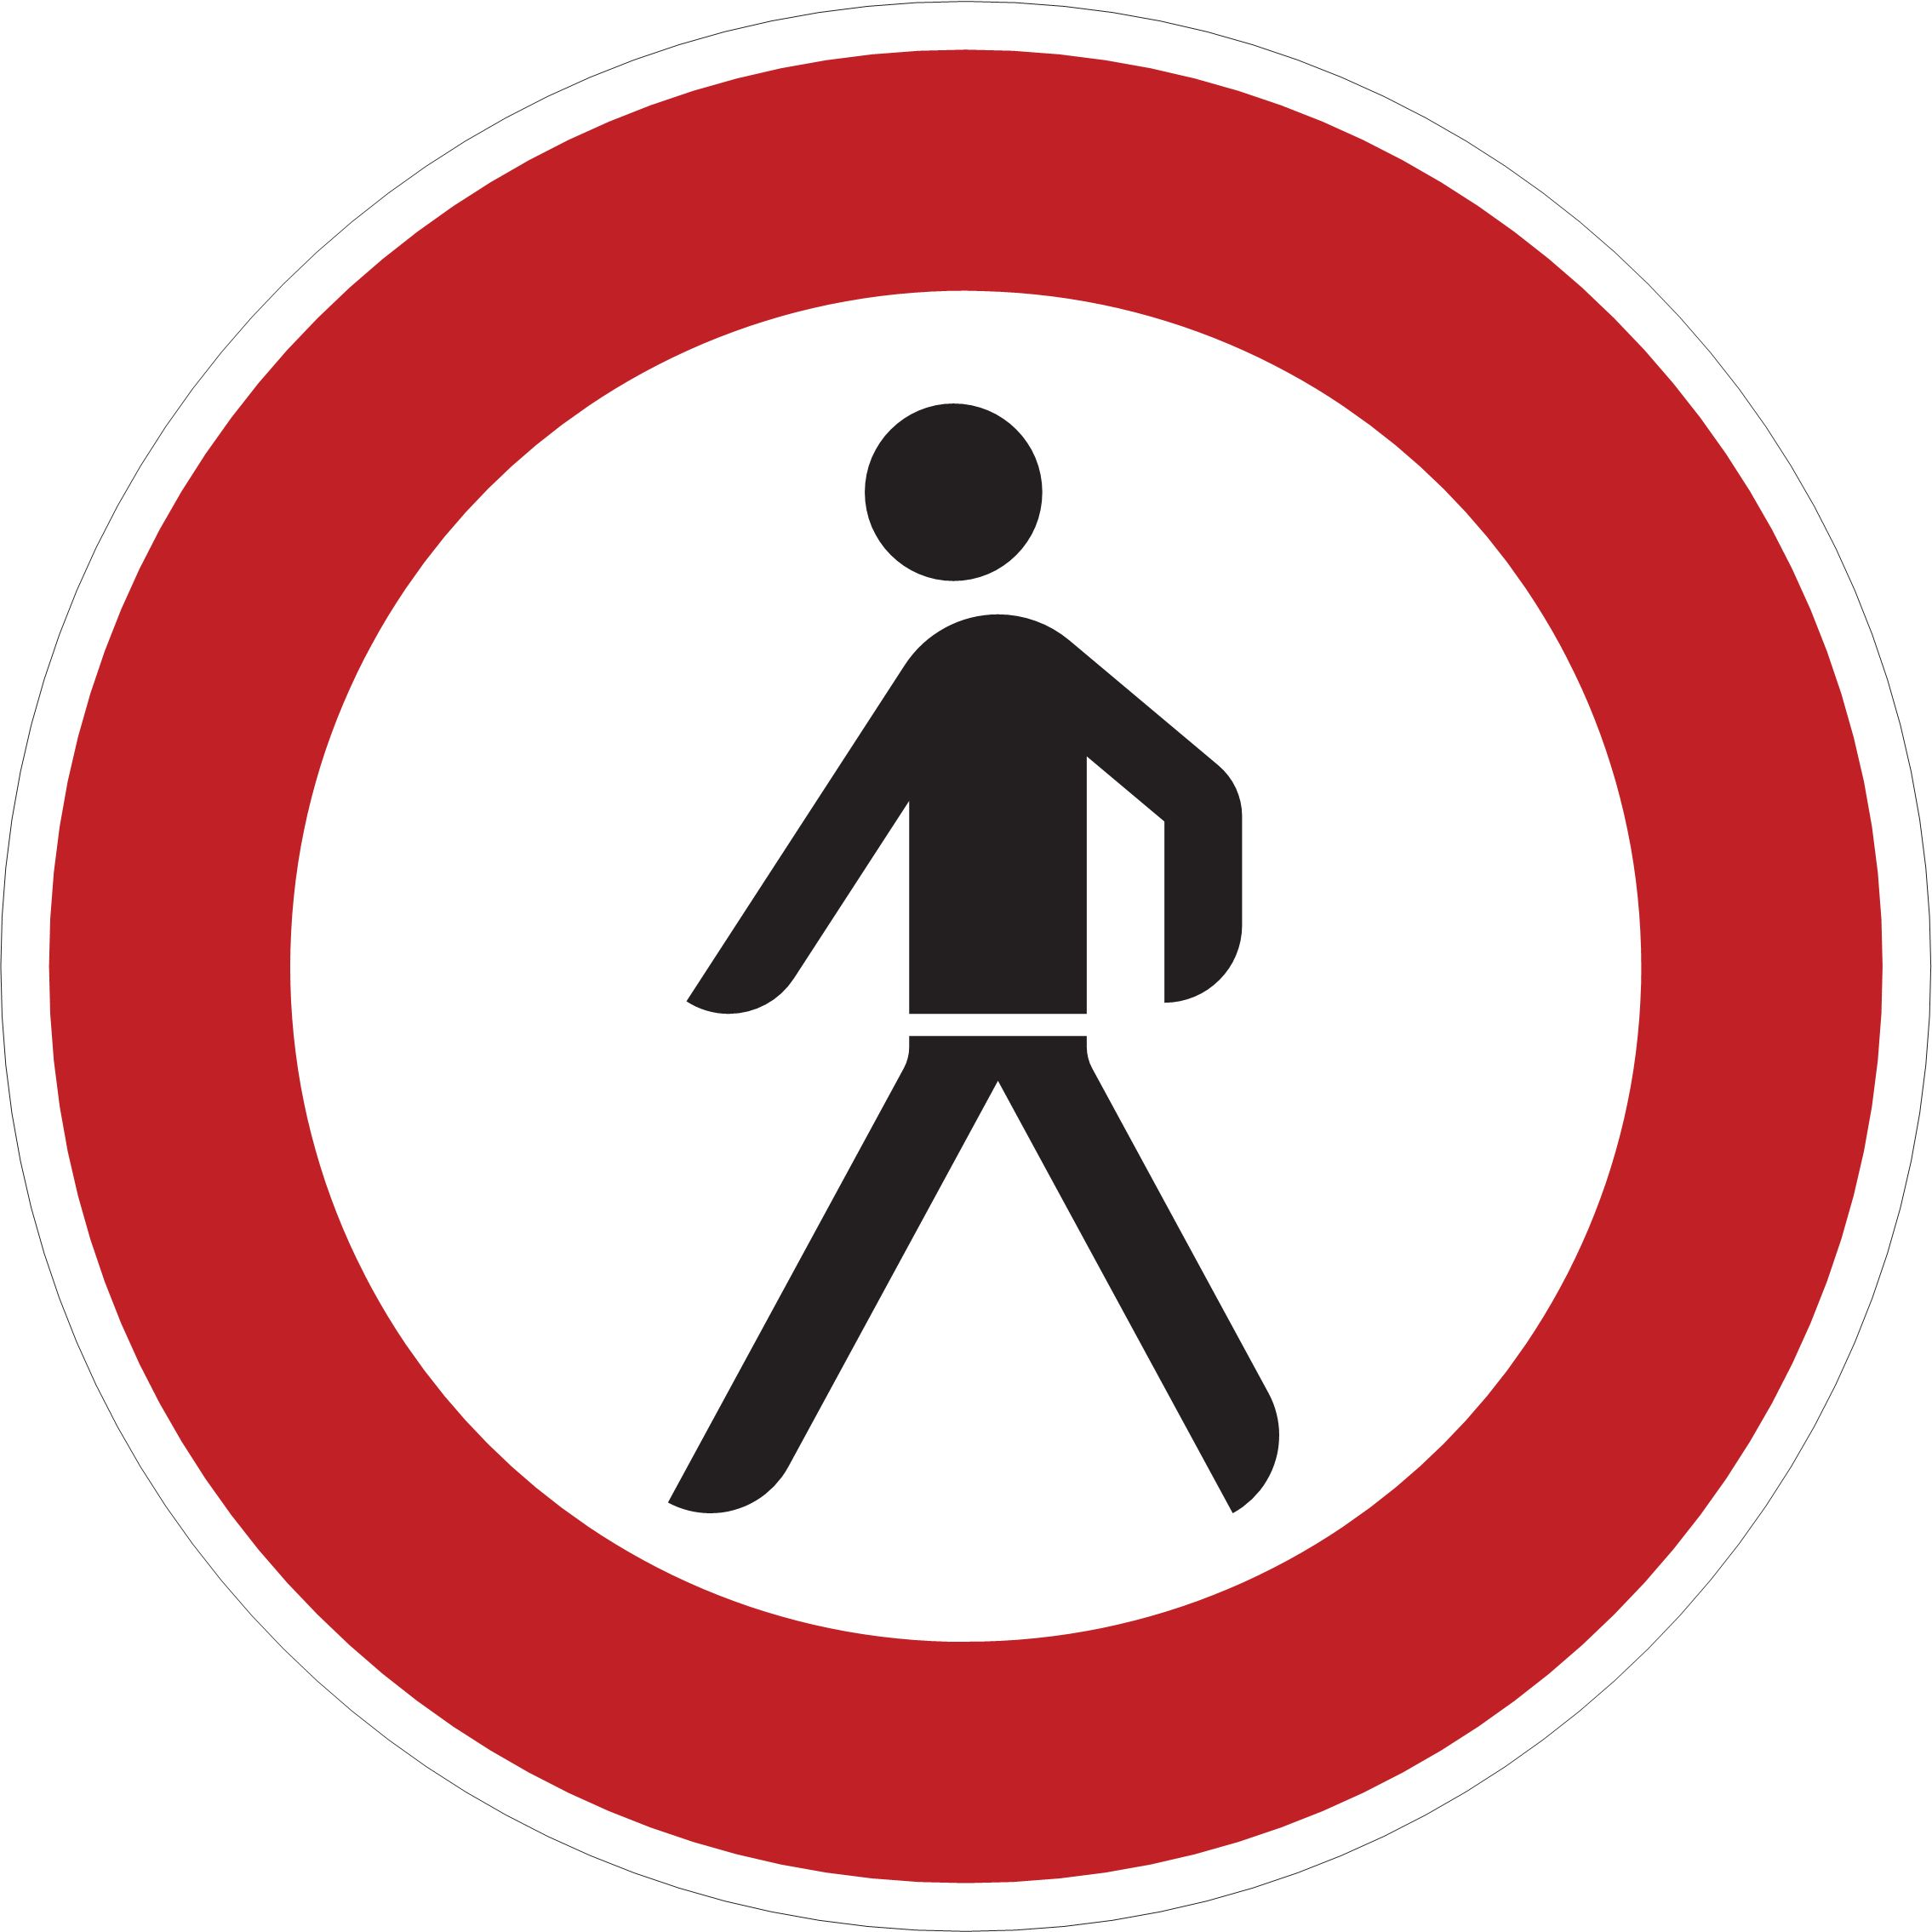
\includegraphics[scale=0.07]{images/PED.jpg}
		\caption{Verbot f\"ur Fu\ss{}g\"anger}
		\label{fig:PED}
	\end{minipage}
	\hfill
	\begin{minipage}[t]{10cm}
		\vspace{0pt}
		\begin{itemize}
			\item Der blau markierte Bereich im Zustandsautomaten beschreibt, was das Schild \glqq Verbot f\"ur Fu\ss{}g\"anger\grqq \ bewirkt. Das Schild wird als "Vorsicht Fu\ss{}g\"anger"\  interpretiert.
			
			\item Wenn als Eingabe \textbf{\textit{PED}} empfangen wird, wird ein Z\"ahler gestartet und das Geschwindigkeitsereignis \textbf{\textit{slow}} ver\"offentlicht.
			
			\item Sobald der Z\"ahler \textbf{\textit{PED\underline{\ }TIME}} \"uberschritten wird, wird das Geschwindigkeitsereignis auf \textbf{\textit{last}} zur\"uckgesetzt und zur\"uck auf den Status \textbf{\textit{DEFAULT}} geschaltet.
		\end{itemize}
	\end{minipage}
\end{figure}


\begin{figure}[h]
	\begin{minipage}[t]{4cm}
		\vspace{0pt}
		\centering
		
\includegraphics[scale=0.04]{images/STOP.jpg}
		\caption{Stoppschild}
		\label{fig:PED}
	\end{minipage}
	\hfill
	\begin{minipage}[t]{10cm}
		\vspace{0pt}
		\begin{itemize}
			\item Der magenta markierte Bereich im Zustandsautomaten beschreibt, was das Schild \glqq Stoppschild\grqq \ bewirkt.
			
			\item Wenn als Eingabe \textbf{\textit{STOP}} empfangen wird, wird ein Z\"ahler gestartet und das Geschwindigkeitsereignis \textbf{\textit{stop}} ver\"offentlicht.
			
			\item Sobald der Z\"ahler \textbf{\textit{STOP\underline{\ }TIME}} \"uberschritten wird, wird das Geschwindigkeitsereignis auf \textbf{\textit{last}} zur\"uckgesetzt. Hierbei wird darauf geachtet, dass der Zustandsautomat erst dann auf \textbf{\textit{DEFAULT}} weiterschaltet, wenn ein Ereignis au\ss{}er \textbf{\textit{STOP}} empfangen wird, um unendliche Schleifen zu vermeiden.
		\end{itemize}
	\end{minipage}
\end{figure}


\begin{figure}[h]
	\begin{minipage}[t]{4cm}
		\vspace{0pt}
		\centering
		
\includegraphics[scale=0.07]{images/40.png}
		\caption{Zul\"assige H\"ochstgeschw.}
		\label{fig:PED}
	\end{minipage}
	\hfill
	\begin{minipage}[t]{10cm}
		\vspace{0pt}
		\begin{itemize}
			\item Der orange markierte Bereich im Zustandsautomaten beschreibt, was das Schild \glqq Zul\"assige H\"ochstgeschwindigkeit 40km/h\grqq\ bewirkt.
			
			\item Wenn als Eingabe \textbf{\textit{40}} empfangen wird, wird das Geschwindigkeitsereignis \textbf{\textit{medium}} ver\"offentlicht.
			
			\item Sobald ein Geschwindigkeitsereignis au\ss{}er \textbf{\textit{40}} empfangen wird schaltet der Zustandsautomat zur\"uck auf den Status \textbf{\textit{DEFAULT}}
		\end{itemize}
	\end{minipage}
\end{figure}


\begin{figure}[h]
	\begin{minipage}[t]{4cm}
		\vspace{0pt}
		\centering
		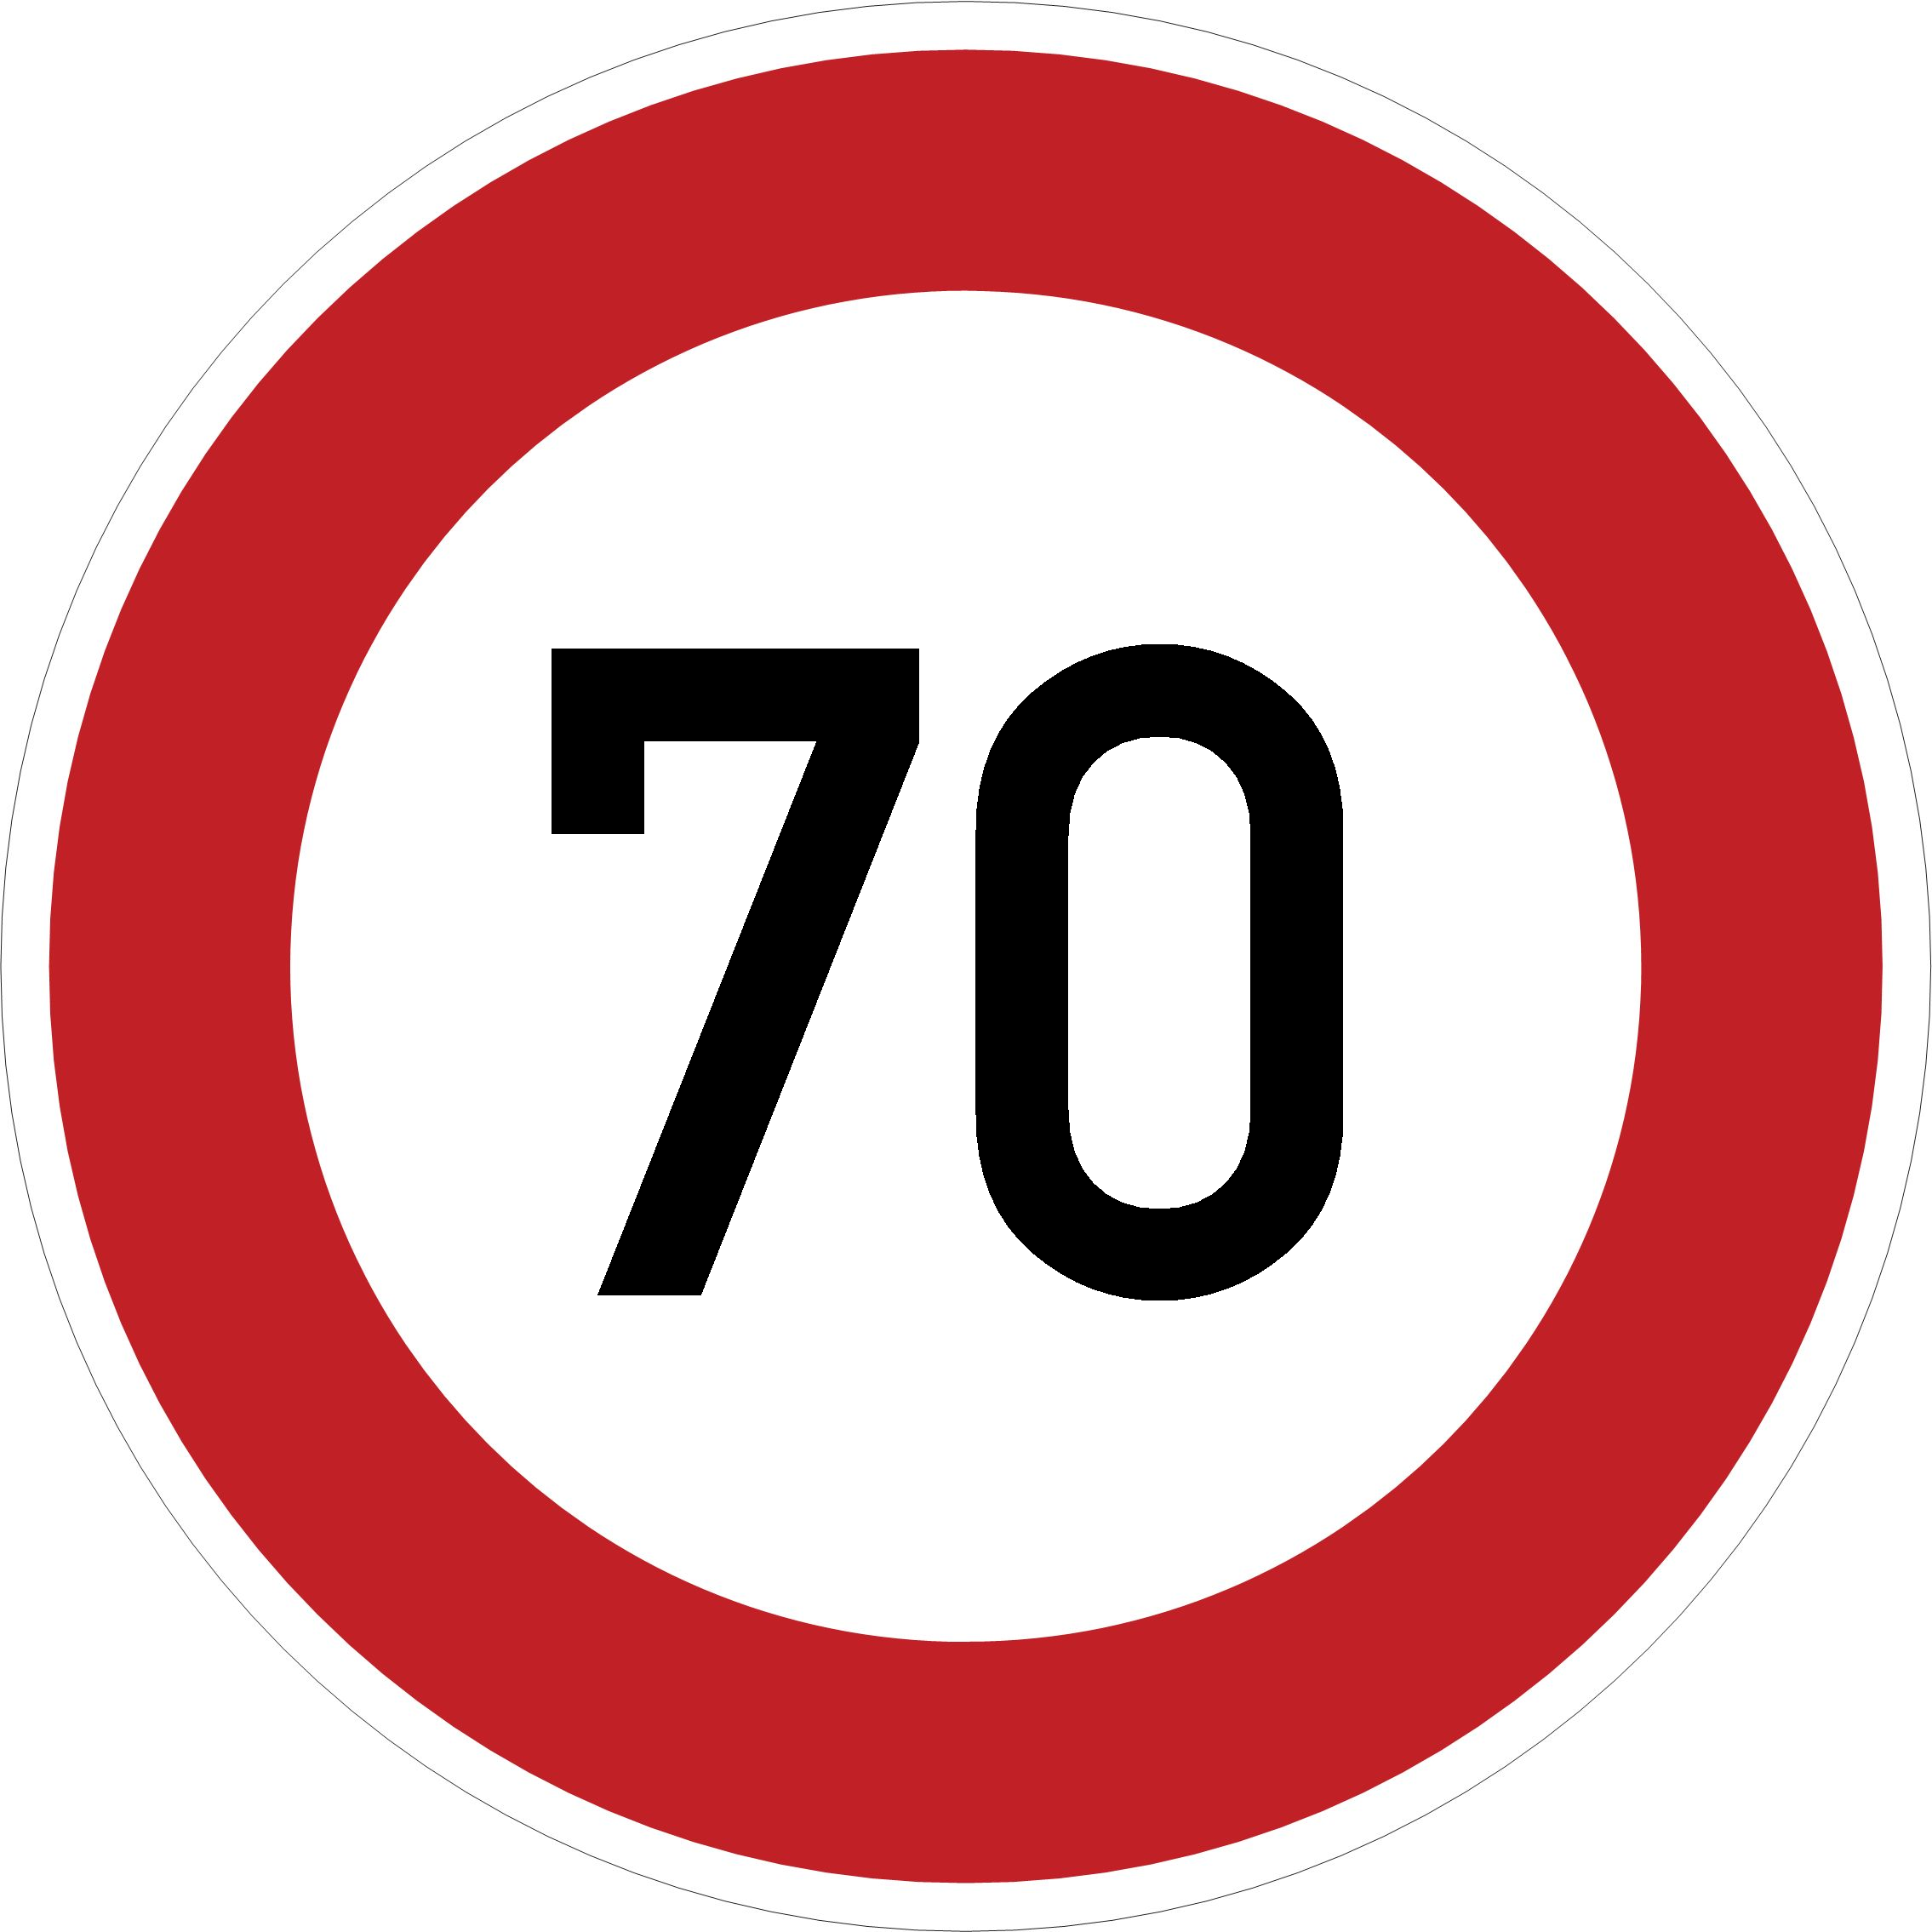
\includegraphics[scale=0.06]{images/70.png}
		\caption{Zul\"assige H\"ochstgeschw.}
		\label{fig:PED}
	\end{minipage}
	\hfill
	\begin{minipage}[t]{10cm}
		\vspace{0pt}
		\begin{itemize}
			\item Der gr\"un markierte Bereich im Zustandsautomaten beschreibt, was das Schild \glqq Zul\"assige H\"ochstgeschwindigkeit 70km/h\grqq \ bewirkt.
			
			\item Wenn als Eingabe \textbf{\textit{70}} empfangen wird, wird das Geschwindigkeitsereignis \textbf{\textit{high}} ver\"offentlicht.
			
			\item Sobald ein Geschwindigkeitsereignis au\ss{}er \textbf{\textit{70}} empfangen wird schaltet der Zustandsautomat zur\"uck auf den Status \textbf{\textit{DEFAULT}}
		\end{itemize}
	\end{minipage}
\end{figure}


